\section{Historical reach on the prescribed geometry grid}\label{sec:reach}
The geometry audit uses the twelve deterministic cells
\begin{equation}
a_\star\in\{0,0.5,0.9,0.98\},\qquad
 i\in\{20^\circ,50^\circ,75^\circ\},\qquad n\in\{0,1,2\}.
\label{eq:geometrygrid}
\end{equation}
The cells are prescribed comparisons, not a random sample from the continuous Kerr parameter space. Each uses the common observer schedule and age grid with its own direct-reference normalization. All numerical values in this section are archived sampled-operator results \cite{archive}.

At $\SNR=100$, adding the first two indirect order-labelled blocks increases the anchor-connected detectable span in every cell. The increase is $40M$ at $20^\circ$, $24M$ at $50^\circ$, and one $4M$ grid step at $75^\circ$. The absolute spans are given in \cref{tab:reach}. At the first two inclinations the anchor is zero. At $75^\circ$ it is $32M$ for zero spin and $28M$ for the three nonzero spins. Thus the high-inclination interval is not a continuous interval starting at age zero.

\begin{table}[htbp]
\centering\small
\caption{Direct and order-labelled anchor-connected scalar-probe spans, in $M$, at $\SNR=100$. The source-independent $4M$ grid limits the resolution of the endpoint. These are detectability spans, not held-out reconstruction spans.}
\label{tab:reach}
\begin{tabular}{c rr rr rr}
\toprule
&\multicolumn{2}{c}{$i=20^\circ$}&\multicolumn{2}{c}{$i=50^\circ$}&\multicolumn{2}{c}{$i=75^\circ$}\\
$a_\star$&Direct&Labelled&Direct&Labelled&Direct&Labelled\\
\midrule
0.00&20&60&60&84&108&112\\
0.50&20&60&60&84&112&116\\
0.90&20&60&60&84&112&116\\
0.98&20&60&60&84&112&116\\
\bottomrule
\end{tabular}
\end{table}

The oldest passing grid centers are $20M$, $60M$, and $140M$ for the direct arm and $60M$, $84M$, and $144M$ for the labelled stack at the three inclinations. Their repetition across sampled spins does not prove spin independence: the anchor-connected values in \cref{tab:reach} already vary with spin. The longest run and anchor-connected run also differ in 316 of the 1152 archived arm--geometry--SNR rows, demonstrating that a single supremum can conceal gaps. Full threshold masks are therefore retained.

\begin{figure}[htbp]
\centering
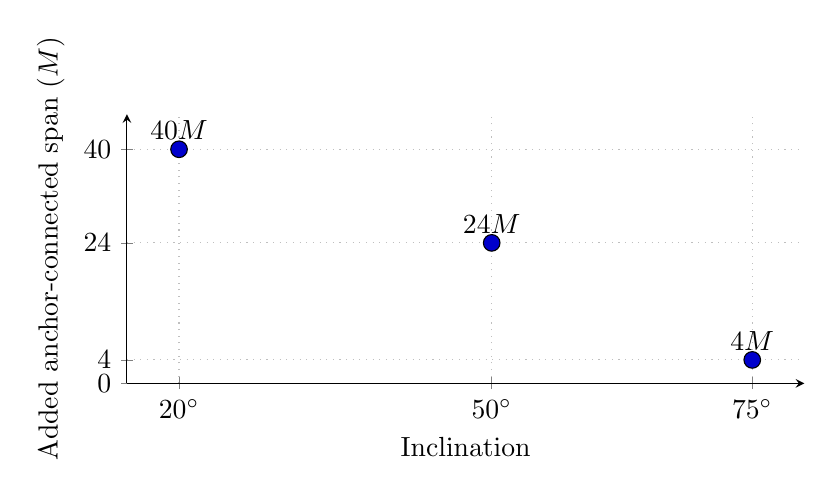
\begin{tikzpicture}
\begin{axis}[width=0.84\linewidth,height=5.0cm,xmin=15,xmax=80,ymin=0,ymax=46,
xtick={20,50,75},xticklabels={$20^\circ$,$50^\circ$,$75^\circ$},
ylabel={Added anchor-connected span ($M$)},xlabel={Inclination},
ytick={0,4,24,40},axis lines=left,clip=false,grid=major,grid style={dotted}]
\addplot+[only marks,mark=*,mark size=3pt,black] coordinates {(20,40)(50,24)(75,4)};
\node[anchor=south] at (axis cs:20,40){$40M$};
\node[anchor=south] at (axis cs:50,24){$24M$};
\node[anchor=south] at (axis cs:75,4){$4M$};
\end{axis}
\end{tikzpicture}
\caption{Incremental scalar-probe span from adding the first two indirect labelled orders. Each marker represents the value shared by four prescribed spin cells, not an average with an inferred population error bar. The $75^\circ$ improvement is one grid quantum. Absolute high-inclination spans still vary with the geometry-specific anchor, as shown in \cref{tab:reach}.}
\label{fig:reach}
\end{figure}

The older twelve-cell spectral audit reports median operational ranks of 153 for direct imaging and 202 for the labelled stack on the global reference class. These counts concern that coefficient representation and threshold, not the nuisance-adjusted compact target of \cref{sec:r2}. The median scalar old-age innovation increases from $8.29M$ to $40.72M$. These observations show additional finite-model sensitivity, but neither count nor innovation measures a recovered movie.

The counterfactual controls reinforce that distinction. The index-sum compression retains a reported median $J_{\rm old}=9.66M$, or $23.7\%$ of the labelled value. This percentage describes the specific compression map, not an unresolved physical image. A pairing-destroyed control retains substantial old-age innovation and can improve conditioning despite breaking the relation between source position, delay, and transfer weight. Similarly, the delay/position substitution statistics, including the archived $0.98$ and $0.57$ comparison, describe index-paired constructions. They cannot establish a physical decomposition of temporal and spatial causes.

\section{Compact support and nuisance-adjusted old-source information}\label{sec:r2}
\subsection{From blind columns to a historical target}
Global temporal modes extend across the source-time interval, so their fitted coefficients alone do not distinguish direct support at an old epoch from inference constrained by a global model. The compact temporal basis makes that support question explicit. At $a_\star=0.5$ and $i=50^\circ$, the original compact-support audit found 84 exactly zero direct columns in the 224-dimensional localized class: three unsupported temporal factors crossed with 28 spatial factors. This is a support statement, not a small-singular-value decision.

The nuisance-adjusted calculation uses a more specific target. It removes the axisymmetric spatial factors from those old compact blocks, giving $3\times4\times6=72$ target coefficients. The remaining 152 coefficients of the full localized 224-dimensional model are unrestricted nuisance coefficients. They include the old axisymmetric contribution, recent-emission factors, and boundary-overlapping temporal factors. Thus ``unknown remainder'' does not mean only an uncertain scalar background.

The target's temporal support lies in approximately $[-128.82,-69.64]M$, outside the retained direct footprint. The direct matrix is identically zero on these columns. This remains true before or after nuisance profiling because zero target response cannot be made informative by projection. The presence of indirect responses is then tested quantitatively, rather than inferred from their nonzero columns.

The distinction from a known-remainder calculation is essential. A nonzero old-target response can still be explained by changing other source coefficients. Equation~\eqref{eq:conditionalfisher} removes every component in that nuisance-response space before counting operational directions. A surviving combination therefore represents likelihood information about this old target conditional on the declared source model, rather than an estimate obtained by fixing the background or extrapolating an assumed source history. The tested remainder is all 152 complementary coefficients; it is not an arbitrary continuum of possible emission fields.

\subsection{Information that survives the unknown remainder}
\Cref{tab:r2} gives the accepted reference-geometry calculation under the frozen legacy screen measure and $\sigma=0.011341986814407566$. The nuisance space has 152 columns; its sampled rank is 140 in the direct arm and 152 in the labelled stack. These ranks are not substituted for target dimension.

\begin{table}[htbp]
\centering\small
\caption{Information for the 72-dimensional old non-axisymmetric target in the full localized 224-dimensional model. The traces use the target source Gram in \eqref{eq:conditionalfisher}. Operational counts use threshold $\rho=1$. All values are for the frozen legacy measure, not a newly qualified common-sky operator.}
\label{tab:r2}
\begin{tabular}{l r r c r}
\toprule
Arm&$\tr F_{\rm known}$&$\tr F_{\rm cond}$&Count: known $\to$ profiled&Nuisance rank\\
\midrule
Direct&0&0&$0\to0$&140\\
Order-labelled&11.053660&7.198318&$3\to2$&152\\
\bottomrule
\end{tabular}
\end{table}

The three largest nuisance-adjusted singular values are
\begin{equation}
1.4371649,\qquad 1.3458733,\qquad 0.8062804.
\label{eq:r2singular}
\end{equation}
Two exceed the operational threshold and the third does not. Profiling preserves approximately $65.12\%$ of the known-remainder Fisher trace. This fraction is a ratio of normalized traces, not a fraction of an independently recovered source history. The count and reported two-dimensional subspace were stable across the three tested nuisance-rank tolerances and the last two source-metric refinements in the accepted replay. Those checks establish numerical stability of this discrete calculation, not uncertainty from a continuum transfer error.

\begin{figure}[htbp]
\centering
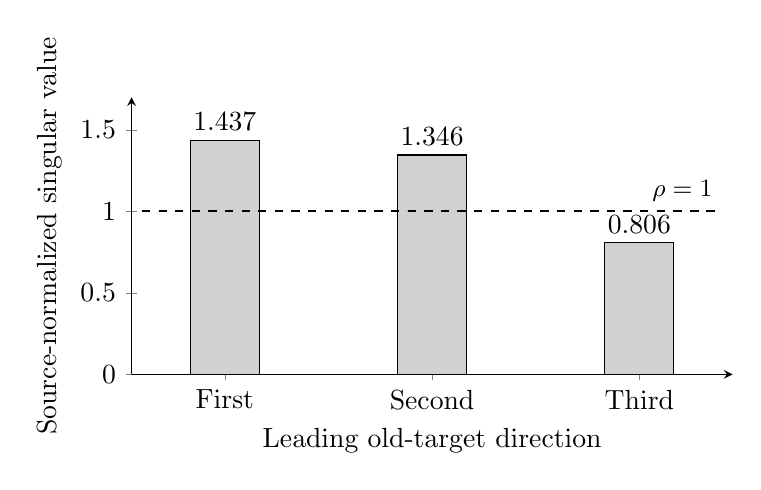
\begin{tikzpicture}
\begin{axis}[width=0.76\linewidth,height=5.1cm,xmin=0.55,xmax=3.45,ymin=0,ymax=1.7,
xtick={1,2,3},xticklabels={First,Second,Third},ylabel={Source-normalized singular value},
xlabel={Leading old-target direction},axis lines=left,clip=false]
\addplot[ybar,bar width=25pt,draw=black,fill=black!18] coordinates {(1,1.4371649)(2,1.3458733)(3,0.8062804)};
\addplot[black,dashed,thick,domain=0.6:3.4] {1};
\node[anchor=south] at (axis cs:1,1.4371649){1.437};
\node[anchor=south] at (axis cs:2,1.3458733){1.346};
\node[anchor=south] at (axis cs:3,0.8062804){0.806};
\node[anchor=south east,font=\small] at (axis cs:3.4,1.0){$\rho=1$};
\end{axis}
\end{tikzpicture}
\caption{The first three singular values after profiling all 152 nuisance coefficients. Two combinations pass the declared threshold under the frozen legacy measure. The direct target response is exactly zero. A separate row-reweighting bound permits one or two passing combinations; this plot is not a corrected-measure recomputation.}
\label{fig:r2}
\end{figure}

Screen-measure changes must be kept separate from the accepted count. The available adopted-cell row-weight ratios span approximately $[0.500081,1.008048]$ across the fixed retained rows; the lower endpoint includes clipped screen-edge cells. Under fixed rows, noise and source metric, the existing reweighting analysis guarantees at least one and at most two operational target directions. It does not establish which count the fully reweighted calculation would attain. Nor does it bound changes from previously unrepresented emitting fragments or a different continuous acquisition. The mathematical reason for the interval is given in Appendix~\ref{app:reweight}; no new spectrum is reported here.

\subsection{Temporal localization in the source norm}
The two surviving modes are signed source perturbations, not images of separate epochs. Their localization must be evaluated after synthesizing the source functions, retaining overlap terms in the Gram matrix. Grouping Cholesky-normalized coordinates by temporal index is not equivalent to integrating energy in physical time windows.

\begin{table}[htbp]
\centering\small
\caption{Squared source-norm fractions of the two operational target modes in disjoint thirds of the old-target interval. The measure is $r\,\dd r\,\dd\phi\,\dd t$, not a proper-volume or prior measure. Values come from the saved source-function localization, not a new mode reconstruction.}
\label{tab:localization}
\begin{tabular}{l r r}
\toprule
Source-time interval ($M$)&Mode 1&Mode 2\\
\midrule
$[-128.82235,-109.09455]$&$2.44\%$&$2.35\%$\\
$[-109.09455,-89.36676]$&$43.81\%$&$43.92\%$\\
$[-89.36676,-69.63897]$&$53.75\%$&$53.73\%$\\
\bottomrule
\end{tabular}
\end{table}

Approximately $97.6\%$ of either mode's source norm lies in the younger two thirds, but the oldest-third contribution is nonzero. The modes are broad and younger-weighted. This finding supports a restricted statement: some old-source information survives an unknown remainder. It does not show independently localized recovery throughout the old interval. The earlier coordinate-weight concentration statistic is not used as a physical-epoch localization.

\section{Source richness separates reach from dimension}\label{sec:stress}
The source-enrichment audit uses three anchors, not the twelve-cell population:
\begin{equation}
(a_\star,i)\in\{(0,20^\circ),(0.5,50^\circ),(0.98,75^\circ)\}.
\label{eq:threeanchors}
\end{equation}
It studies four spaces with radial, azimuthal, and temporal dimensions $(4,7,8)$, $(4,7,16)$, $(6,11,8)$, and $(6,11,16)$. These form temporal and spatial branches, not a single monotonically ordered temporal ladder. Refining radial knots changes individual spline columns; the recorded nesting check concerns function-space containment. Its worst parent-to-child projection residual is $2.73\times10^{-14}$.

\begin{table}[htbp]
\centering\small
\caption{Archived order-labelled source-class summaries over the three prescribed anchors. Operational rank and its dimension-normalized fraction are distinct from numerical rank. The smallest positive singular values use the archived coefficient-operator convention. These are not the nuisance-adjusted counts in \cref{tab:r2}.}
\label{tab:enrichment}
\begin{tabular}{l c r r r r}
\toprule
Class&Factors&Dimension&Median operational rank&Fraction&$\sigma_{\min}^{+}$\\
\midrule
\texttt{C224}&$4\times7\times8$&224&201&0.897&$1.635\times10^{-2}$\\
\texttt{C448\_T}&$4\times7\times16$&448&365&0.815&$7.164\times10^{-5}$\\
\texttt{C528\_S}&$6\times11\times8$&528&441&0.835&$2.871\times10^{-4}$\\
\texttt{C1056\_ST}&$6\times11\times16$&1056&770&0.729&$1.332\times10^{-7}$\\
\bottomrule
\end{tabular}
\end{table}

From the first to the richest class, the median operational fraction decreases by about 16.8 percentage points, while its absolute count increases from 201 to 770. The fraction is not monotone across the listed branches: the spatial-only enrichment has a higher fraction than the temporal-only enrichment. The smallest positive singular value decreases by roughly five orders of magnitude across the full comparison. Source enrichment exposes more poorly supported questions; it does not universally reduce the number of supported directions or imply loss of every identifiable component.

At the reconstruction anchor, the direct numerical ranks across the four classes are 224, 411, 528, and 911; the labelled ranks are 224, 448, 528, and 1045. The localized-directional reach there remains $60M$ for the direct arm and $92M$ for the labelled arm in each class. These values differ from the scalar-probe $60M/84M$ comparison because the probe families differ.

Across the physical and mechanism arms at the three anchors, the directional endpoints move by at most one $4M$ grid step, with observed changes at spatial-enrichment steps and none at the temporal steps. The nonphysical permutation arm has a larger exceptional shift and is not evidence of physical reach. These are model-specific observations, not a general theorem assigning reach exclusively to spatial or temporal complexity.

\begin{figure}[htbp]
\centering
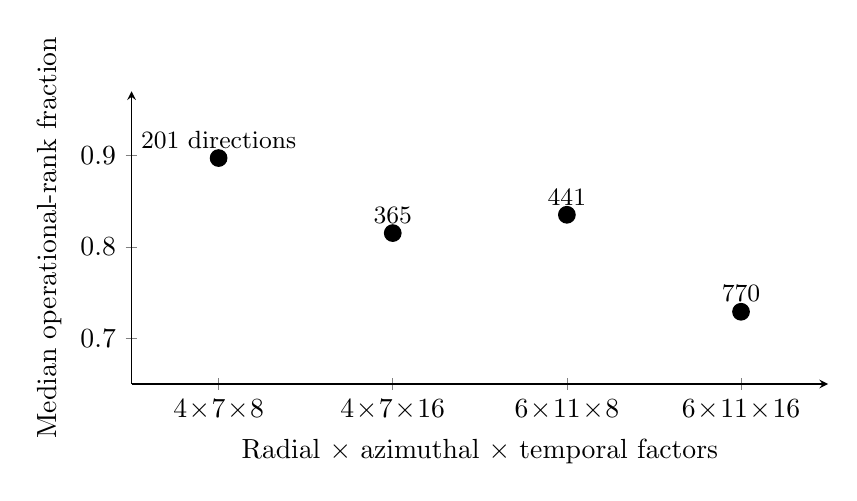
\begin{tikzpicture}
\begin{axis}[width=0.86\linewidth,height=5.3cm,ymin=0.65,ymax=0.97,
xtick={1,2,3,4},xticklabels={$4\!\times\!7\!\times\!8$,$4\!\times\!7\!\times\!16$,$6\!\times\!11\!\times\!8$,$6\!\times\!11\!\times\!16$},
xmin=0.5,xmax=4.5,ylabel={Median operational-rank fraction},
xlabel={Radial $\times$ azimuthal $\times$ temporal factors},axis lines=left,clip=false]
\addplot[only marks,mark=*,mark size=3pt,black] coordinates {(1,0.897)(2,0.815)(3,0.835)(4,0.729)};
\node[anchor=south,font=\small] at (axis cs:1,0.897){201 directions};
\node[anchor=south,font=\small] at (axis cs:2,0.815){365};
\node[anchor=south,font=\small] at (axis cs:3,0.835){441};
\node[anchor=south,font=\small] at (axis cs:4,0.729){770};
\end{axis}
\end{tikzpicture}
\caption{Supported fraction and absolute supported count need not move together. Points summarize the order-labelled operator over the three E3D anchors. The middle two classes are alternative enrichment branches, so no interpolating line or monotone trajectory is asserted. The source of each plotted number is \cref{tab:enrichment}.}
\label{fig:enrichment}
\end{figure}
\FloatBarrier
